\documentclass{beamer}
\usepackage[utf8]{inputenc}
\usepackage[danish]{babel}
\usepackage{amsmath}
\usepackage{graphicx}

\usetheme{Warsaw}
\usecolortheme{lily}


\begin{document}
\title[Aktivitet - Forstærker]
{Aktivitet - Forstærker}
\subtitle{E-EEP (Elektromagnetisme, Elektronik og Projekt) og E-RMK (Regulering, Matematik og Kredsløbsteknik) E16}
\author[Gruppe 4] % (optional, for multiple authors)
{Gruppe 4\\ 
J\"{o}rn Jacobi, Simon Juul M\o ller\\ S\o ren Frank, Kenneth Petersen\\ Nikolaj Kyed, Benjamin Lund}
\institute{ 
  %
\includegraphics[height=2cm]{images/sdu_logo2.png}\\
  M\ae rsk Mc-Kinney M\o ller Instituttet \\
  Syddansk Universitet
}
\date{17/11-2016}
%\subject{Elektromagnetisme, Analog signal behandling og Reguleringsteknik}
\logo{
\includegraphics[height=1cm]{images/sdu_logo2.png}}

\frame{\titlepage}

%\begin{frame}
%	\frametitle{Indhold}
%	\tableofcontents[currentsection]
%\end{frame}

%\section{Oplæg til stormøde}
\begin{frame}
	\frametitle{Topologi valg}
	Fællesemitter med delvis afkobling over emitter-modstanden ($R_{E2}$).
	\begin{center}
		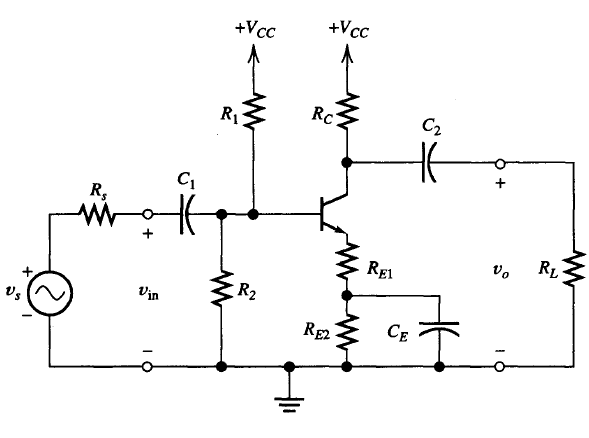
\includegraphics[width=0.8\linewidth]{images/trans_topo1.png}
	\end{center}
\end{frame}

\begin{frame}
	\frametitle{Topologi valg - Krav}
	\begin{center}
		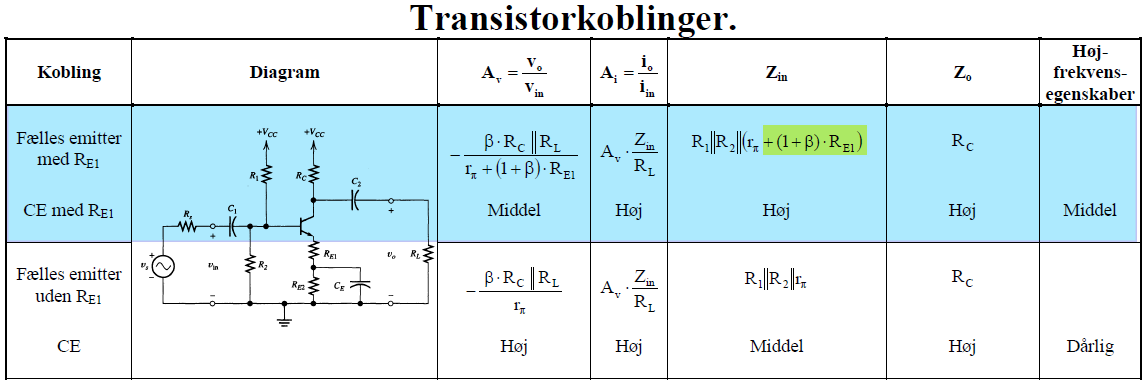
\includegraphics[width=1\linewidth]{images/trans_topo2.png}
	\end{center}
	\begin{itemize}
		\item $Z_i \geq  5 kHz$ i frekvensområdet $20 Hz - 20 kHz$
		\item $A_V = \dfrac{v_o}{v_i} = -20 \pm 2$
	\end{itemize}
\end{frame}

\begin{frame}
	\frametitle{Beregninger I}
	\begin{columns}[onlytextwidth]
  \begin{column}{0.4\textwidth}
    \begin{center}
		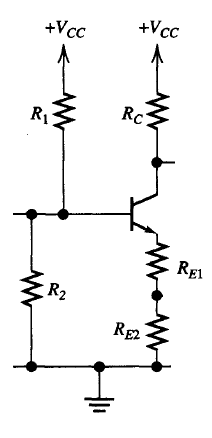
\includegraphics[width=.8\textwidth]{images/trans_dc.png}
	\end{center}
  \end{column}
  \begin{column}{0.6\textwidth}
  	Valg:
    \begin{itemize}
	\item $I_{RC} = 8 mA$
	\item $V_{cc} = 15 V$ fordelt lige over $R_C$, $V_{CE}$ og $R_{E1}+R_{E2}$ \footnote{Se side 245 i lærebogen}
	\item $I_{R2} \simeq 10\cdot I_B$ 
	\end{itemize}
  \end{column}
\end{columns}
\end{frame}

\begin{frame}
	\frametitle{Beregninger II}
	\begin{columns}[onlytextwidth]
  \begin{column}{0.4\textwidth}
    \begin{center}
		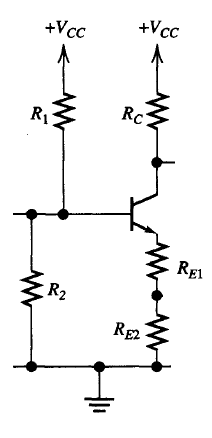
\includegraphics[width=.8\textwidth]{images/trans_dc.png}
	\end{center}
  \end{column}
  \begin{column}{0.6\textwidth}
	Beregninger:
	\begin{itemize}
	\item $R_C = \frac{V_{RC}}{I_{RC}}= \frac{5V}{8mA} = 625\Omega$
	\item $I_B = \frac{I_C}{\beta} = \frac{8mA}{290}=27.59\mu A $ \footnote{Datablad for BC547B}
	\item $R_E = \frac{V_{RE1+RE2}}{I_B+I_C} = 622\Omega $
	\item $V_{R2} = V_{BE} + V_{RE} = 5,7V$
	\item $I_{R2} = 8\cdot I_B$
	\item $R_2 = \frac{V_{R2}}{I_{R2}} = 25.82k\Omega $
	\item $R_1 = \frac{V_{cc}-V_{R2}}{I_{R2}+I_B} = 29.12k\Omega$
	\item $r_{\pi} = \frac{\beta \cdot V_T}{I_C}$
	\item $A_v = - \frac{\beta \cdot R_C || R_L}{r_{\pi}+(1+\beta)\cdot R_{E1}} = 20$
	\item $R_E = R_{E1} + R_{E2} = 622\Omega$
	\item $\Rightarrow R_{E1}= 26.07\Omega \wedge R_{E2}=597\Omega$
	\end{itemize}		
  \end{column}
\end{columns}
\end{frame}

\begin{frame}
	\frametitle{Beregninger III - AC analyse}
	\begin{columns}[onlytextwidth]
  \begin{column}{0.4\textwidth}
    \begin{center}
		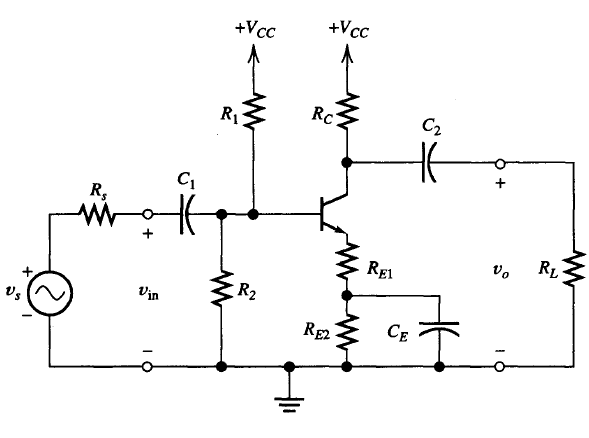
\includegraphics[width=1\textwidth]{images/trans_topo1.png}
	\end{center}
  \end{column}
  \begin{column}{0.6\textwidth}
	Beregninger:
	\begin{itemize}
	\item $Z_i = R_1||R_2||(r_{\pi}+(1+\beta)\cdot R_E1) = 5,15k\Omega$
	\item $Z_o = R_C = 625\Omega$
	\item $C_1 = \frac{1}{2\cdot \pi \cdot f \cdot Z_{i}+R_{s}}$
	\item $\Rightarrow C_1= 3,00\mu F$ ved $20Hz$
	\item $C_2 = \frac{1}{2\cdot \pi \cdot f \cdot Z_{o}+R_{L}}$
	\item $\Rightarrow C_2= 1,50\mu F$ ved $20Hz$
	\item $C_E \sim \beta \cdot C_1$\footnote{Se side 542}
	\end{itemize}
	Hver kondensator giver et $3dB$ bidrag ved ønsket frekvens. Alle kondensatorer tilpasses ved PSpice simuleringen. 
  \end{column}
\end{columns}
\end{frame}

\begin{frame}
	\frametitle{Komponent valg}
	\begin{itemize}
		\item Alle modstande tilpasses til nærmeste standard R12 værdi SMD. 
		\item  $C_1$, $C_2$ er valgt som SMD
		\item $C_E$ vælges som elektrolyt pga. pris
		\item Afkoblings kondensatorerne tilpasser efter PSpice analyse og valg mht. hvad der er nødvendigt og tilgængeligt på lager.
		\item BC547A anvendes i stedet for BC547B.  
	\end{itemize}
\end{frame}

\begin{frame}
	\frametitle{PSpice design}
	\begin{center}
		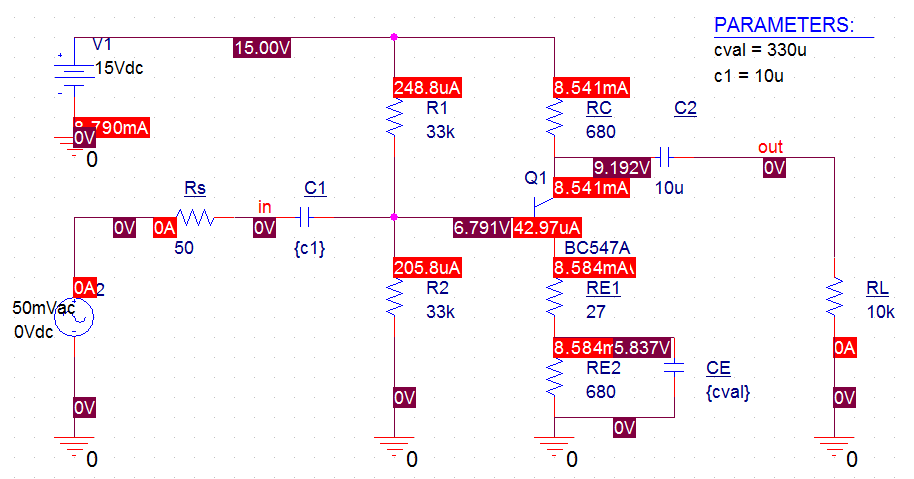
\includegraphics[width=1\textwidth]{images/pspice.png}
	\end{center}	
\end{frame}

\begin{frame}
	\frametitle{PSpice simulering}
	\begin{center}
		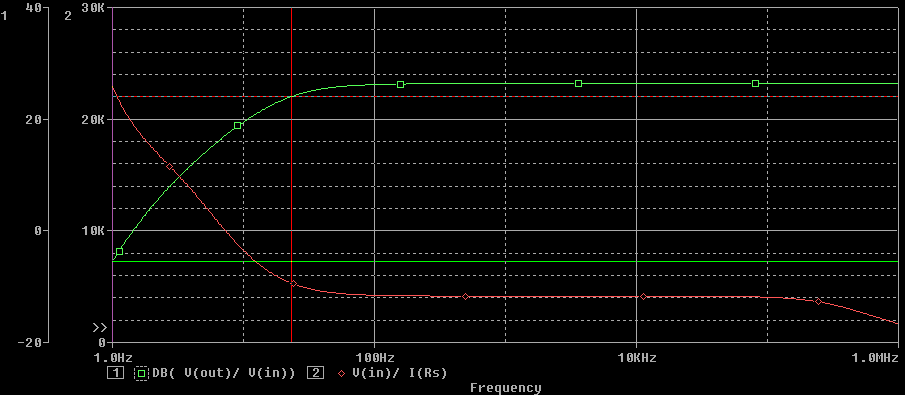
\includegraphics[width=1\textwidth]{images/pspice_plot.png}
	\end{center}
\end{frame}

\begin{frame}
	\frametitle{Måleskema}
	\begin{center}
		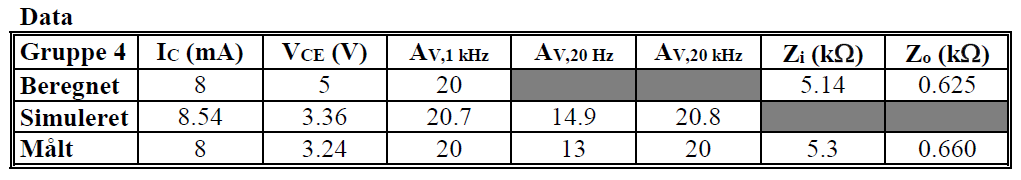
\includegraphics[width=1\textwidth]{images/data.png}
	\end{center}	
\end{frame}

\begin{frame}
	\frametitle{Stykliste}
	\begin{center}
		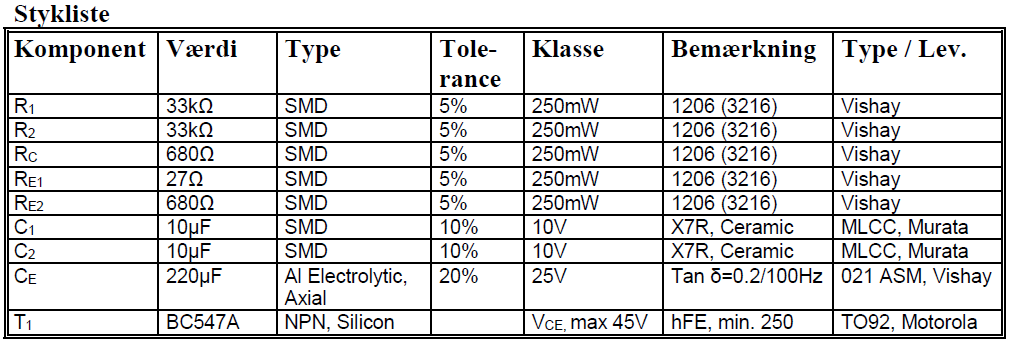
\includegraphics[width=1\textwidth]{images/stykliste.png}
	\end{center}	
\end{frame}

\begin{frame}
	\frametitle{Spørgsmål}
\begin{center}
		
\includegraphics[width=0.7\linewidth]{images/q.jpg}
	\end{center}
\end{frame}

\end{document}

\section{x}
\begin{frame}
	\frametitle{x}
	\begin{itemize}
	\item x
	\end{itemize}	
\end{frame}

% Remove this frame at the end
\begin{frame}
	\frametitle{only ref.}

	\begin{itemize}
		\item Item 1
		\item Item 2
	\end{itemize}
	
	\begin{block}{This is a Block}
		This is important information
	\end{block}
	
	\begin{alertblock}{This is an Alert block}
		This is an important alert
	\end{alertblock}

   	\begin{exampleblock}{This is an Example block}
   		This is an example 
   	\end{exampleblock}
   
	\begin{center}
		
\includegraphics[width=1in]{images/sdu_logo2.png}
	\end{center}

\end{frame}


